\documentclass[11pt]{article}
    \title{\textbf{Math 217 Homework I}}
    \author{Khac Nguyen Nguyen}
    \date{}
    
    \addtolength{\topmargin}{-3cm}
    \addtolength{\textheight}{3cm}
    
\usepackage{amsmath}
\usepackage{mathtools}
\usepackage{amsthm}
\usepackage{amssymb}
\usepackage{pgfplots}
\usepgfplotslibrary{polar}
\usepgflibrary{shapes.geometric}
\usetikzlibrary{calc}
\pgfplotsset{compat = newest}
\pgfplotsset{my style/.append style = {axis x line = middle, axis y line = middle, xlabel={$x$}, ylabel={$y$}, axis equal}}
\begin{document}
\section*{1.}
(i) the set $ A = \{ (x,y) \in \mathbb{R}^2: x>y \}$ is convex:
\begin{equation*}
\begin{aligned}
\forall m = (x_1,y_1), n=(x_2,y_2) \in A: tm+ (1-t)n &= (tx_1, ty_1) + (x_2-tx_2, y_2 -ty_2) \\
&= (tx_1+x_2-tx_2,ty_1+y_2 - ty_2)
\end{aligned}
\end{equation*}
\begin{equation*}
\begin{aligned}
\forall t \in [0,1]: &tx_1+x_2-tx_2 - ty_1 -y_2 + ty_2 = \underbrace{t}_{>0} \underbrace{(x_1-y_1)}_{>0} + \underbrace{(1-t)}_{>0} \underbrace{(x_2 - y_2)}_{>0} > 0 \\
\implies & x_1+x_2-tx_2 > ty_1+y_2 -ty_2 \implies tm+(1-t)n \in A
\end{aligned}
\end{equation*}	
(ii) the set $B= \{x \in \mathbb{R}^N: \|x\|>2\} $ is not convex: \\
Consider $x = (3,0, \ldots, 0), y = (-3,0, \ldots, 0) \in B \text{ as } \|x\|= \|y\| = 3 $ \\
If $t=\cfrac{1}{2} \in [0,1]$, then 
\begin{equation*}
\begin{aligned}
\|tx+(1-t)y\| &= \left\|\left(\cfrac{1}{2} \cdot 3, 0, \ldots, 0\right) + \left(\cfrac{1}{2} \cdot (-3), 0, \ldots, 0\right) \right\| \\
&= \|(0,0,\ldots, 0)\| = 0.
\end{aligned}
\end{equation*}
Therefore,  $tx+(1-t)y \notin B$. \\
(iii) the set $C = \mathbb{R} \backslash \mathbb{Q} $ is not convex:
Consider $\pi, -\pi \in C$ \\
If $t=\cfrac{1}{2}$, then $t\pi + (1-t)\pi = 0 \notin C$. \\
(iv) the set $ D = \{ (x,y,z) \in \mathbb{R}^3: x+y+z\ge 2022\}$ is convex:
\[\forall m = (x_1,y_1,z_1), n=(x_2,y_2,z_2) \in A: \]
\begin{equation*}
\begin{aligned}
\forall t \in [0,1]: tm+ (1-t)n &= (tx_1, ty_1, tz_2) + (x_2-tx_2, y_2 -ty_2, z_2 - ty_2) \\
&= (tx_1+x_2-tx_2,ty_1+y_2 - ty_2, tz_1+z_2 - tz_2) \\
&=tx_1+x_2-tx_2+ty_1 +y_2 - ty_2 + tz_1 + z_2 -tz_2 \\
&= \underbrace{t}_{>0} \underbrace{(x_1+y_1+z_1)}_{\ge 2022} + (1-t) \underbrace{(x_2+ y_2+z_2)}_{>0} \\ 
&\ge  t \cdot 2022 + (1-t) \cdot 2022 = 2022 \\
&\implies tm+(1-t)n \in D
\end{aligned}
\end{equation*}	
\pagebreak
\section*{2.}
Let $\mathcal{C} = \{C_i | i \in I \}$ be the family of convex sets, then
\[\forall x,y \in \bigcap_{C \in \mathcal{C}} C: x,y \in C_i \forall i \in I\]
and since $C_i$ is convex for all $i \in I$, which means that
\[
\forall t \in [0,1]: tx + (1-t)y \in C_i \, \forall i \in I 
\]
Therefore, 
\[
tx+(1-t)y \in \bigcap_{C \in \mathcal{C}} C
\]
and hence $\bigcap_{C \in \mathcal{C}} C$ is also convex.\\
However, $\bigcup_{C \in \mathcal{C}} C$ is not necessarily convex: \\
Consider the two convex sets $B_1[1,0] \text{ and } B_1[-1,0] \in \mathbb{R}^2$. \\
The point $x = (1,-1) \in B_1[1,0]$ since $\| (1,-1) - (1,0)\| = 1$ \\
and the point $y = (-1,-1) \in B_1[-1,0]$ since $\| (-1,-1) - (-1,0)\| = 1$
but given $t= \cfrac{1}{2}, tx+(1-t)y = \left(\cfrac{1}{2}, -\cfrac{1}{2}\right) + \left(-\cfrac{1}{2}, -\cfrac{1}{2}\right)  = (0, -1)$ \\
$\|(1,0) - (0,-1)\| = \sqrt{2}$ and $\|(-1,0) - (0,-1)\| = \sqrt{2}$. Therefore $tx+(1-t)y \notin B_1[1,0] \cup B_1[-1,0]$
\pagebreak
\section*{3.}
Consider an open interval $\forall n \in \mathbb{Z}: (n,n+1)$ is open, then $\bigcup_{n \in \mathbb{Z}}(n,n+1)$ is also open. We have
\[\forall r \in \mathbb{R}: \exists n \in \mathbb{Z}, \exists 0 \le m < 1 \in \mathbb{R}: r = n+m \]
If $m\ne 0$ then $r \in (n,n+1)$ \\
else if $m=0$ then $r \in \mathbb{Z}$ as $n=r$. \\
Therefore, $R \backslash \bigcup_{n \in \mathbb{Z}}(n,n+1) = \mathbb{Z}$ and consequently, $\mathbb{Z}$ is closed in $\mathbb{R}$. \\
Consider $0 \in \mathbb{Z}, \forall \epsilon >0: \exists n: \frac{1}{n} < \epsilon \land \frac{1}{n} < 1 $ and therefore, $\frac{1}{n} \in B_\epsilon(0)$ which means that $\forall \epsilon >0: B_\epsilon{0} \not\subset \mathbb{Z}$ and hence $\mathbb{Z}$ is not open. \\ 
Suppose $\mathbb{Q}$ is open, then given $q \in \mathbb{Q}: \exists \epsilon >0: (q-\epsilon, q+\epsilon) \subset \mathbb{Q}$. \\
But $\forall \epsilon >0$, there exists an $n$ large enough so that $\cfrac{\sqrt{2}}{n} < \epsilon$ and therefore $q+ \cfrac{\sqrt{2}}{n}$ is irrational and is an element of $(q-\epsilon, q+\epsilon)$ which is a contradiction. Therefore $\mathbb{Q}$ is not open. \\
Suppose $\mathbb{Q}$ is closed, then $\mathbb{R} \backslash \mathbb{Q}$ is open, which means for a given $x \in \mathbb{R} \backslash \mathbb{Q}: \exists \epsilon: (x-\epsilon, x+\epsilon) \subset \mathbb{R} \backslash \mathbb{Q}$.\\
But for all open interval, there exists a rational number in that interval, which means that there is $y \in \mathbb{Q} \land y \in (x-\epsilon, x+\epsilon)$ which is a contradiction. \\
Therefore $\mathbb{Q}$ is not closed.
\pagebreak
\section*{4.}
$\forall t \in S+U: t = x+y$ where $x\in S \land y \in U$. \\
Since $y \in U: \exists \epsilon >0: B_\epsilon(y) \in U$ \\
$\forall t' \in B_\epsilon(t), \text{ let } t' = t+d$, then
\[
\|t' - t\| = \| d \| < \epsilon
\]
Let $y' = y+d$, then
\[
\|y'-y\| = \| d \| < \epsilon
\]
which means that $y' \in U$ and $t' = x + y'$ where $x\in S \land y' \in U$. \\
As a result, $\forall t' \in B_\epsilon(t): t' \in S+U$ and hence $B_\epsilon(t) \in S+U$. \\
Therefore, $S+U$ is open
\pagebreak
\section*{5.}
Given $x \in \mathbb{R}^N$ is a cluser point of $x$, if there is a neighborhood of $x$ contains finite points of $S$, which means that
\[
\exists \epsilon >0: B_\epsilon(x) \cap S = \{ x_1, x_2, \ldots, x_n\} 
\]
Since the set has finite element, the set $T = \{\| x-x_i\| | i\in \{1,2,\ldots, n\}\}$ also has finite element and therefore has a minimum which we denote $\delta$. Then 
\[(B_\delta(x) \cap S )\backslash \{x\}= \O\]
which means that $x$ is not a cluster point and therefore leads to a contradiction. Therefore, the neighborhood of $x$ must contain infinite elements. \\
If each neighborhood of $x$ contains an infinte number of points in $S$ then $x$ is obviously a cluster point
\pagebreak
\section*{6.}
a. \\
(i) 
\[
\| x\|_1 = \underbrace{|x_1|}_{\ge 0} + \underbrace{|x_2|}_{\ge 0} + \ldots + \underbrace{|x_N|}_{\ge 0}\ge 0
\]
\[
\| x\|_\infty = \text{max}\{\underbrace{|x_1|}_{\ge 0}, \underbrace{|x_2|}_{\ge 0}, \ldots,  \underbrace{|x_N|}_{\ge 0} \} \ge 0
\]
If $x \ne 0$, then $\exists i: x_i \ne 0$, which means that 
\[
\|x\|_1 = \underbrace{|x_1|}_{\ge 0} + \underbrace{|x_2|}_{\ge 0} + \ldots + \underbrace{|x_i|} + \ldots + \underbrace{|x_N|}_{\ge 0}\ge |x_i| > 0 
\]
\[
\| x\|_\infty = \text{max}\{|x_1|, |x_2|, \ldots, |x_N|\} \ge |x_i| >0
\]
Therefore, $\|x\|_1 = 0 \implies x=0$ and $\|x\|_\infty = 0 \implies x=0$ \\
It is also obvious that if $x=0$, then
\[
\| x\|_1 = \underbrace{|x_1|}_{= 0} + \underbrace{|x_2|}_{= 0} + \ldots + \underbrace{|x_N|}_{=0}= 0
\]
and
\[
\| x\|_\infty = \text{max}\{\underbrace{|x_1|}_{= 0}, \underbrace{|x_2|}_{= 0}, \ldots,  \underbrace{|x_N|}_{= 0} \} = 0
\]
(ii)
\begin{equation*}
\begin{aligned}
\|\lambda x\|_1 &=  |\lambda x_1| + |\lambda x_2| + \ldots + |\lambda x_N| \\
&= |\lambda||x_1| + |\lambda||x_1| + \ldots + |\lambda||x_1| \\
&= |\lambda| (|x_1| + |x_2| + \ldots + |x_N|) =  |\lambda|\|x\|_1 \\
\|\lambda x\|_\infty &=  \text{max}\{|\lambda x_1| , |\lambda x_2| , \ldots , |\lambda x_N| \} \\
&= \text{max} \{|\lambda||x_1|, |\lambda||x_1|, \ldots , |\lambda||x_1| \}\\
&= |\lambda |\text{max} \{|x_1|, |x_2|, \ldots, |x_N|\} \\
&= |\lambda| \|x\|_\infty
\end{aligned}
\end{equation*}
(iii)
\begin{equation*}
\begin{aligned}
\| x+y\|_1 &= |x_1 + y_1| + |x_2 + y_2| + \ldots + |x_N + y_N| \\
& \le |x_1| + |y_1| + |x_2| + |y_2| + \ldots + |x_N| + |y_N| \\
&= \|x\|_1 + \|y\|_1 \\
\|x+y\|_\infty &=  \text{max}\{ |x_1 + y_1| + |x_2 + y_2| + \ldots + |x_N + y_N|\}\\
&\le \text{max} \{  |x_1| + |y_1|, |x_2| + |y_2|, \ldots , |x_N| + |y_N| \} \\
&\le \text{max} \{ |x_1|, |x_2|, \ldots, |x_N|\} + \text{max}\{|y_1|, |y_2|, \ldots ,|y_N|\} \\
&= \|x\|_\infty + \|y\|_\infty
\end{aligned}
\end{equation*}
\\~\\
b. \\
For $\|x\|_1 \le 1$: \\ 
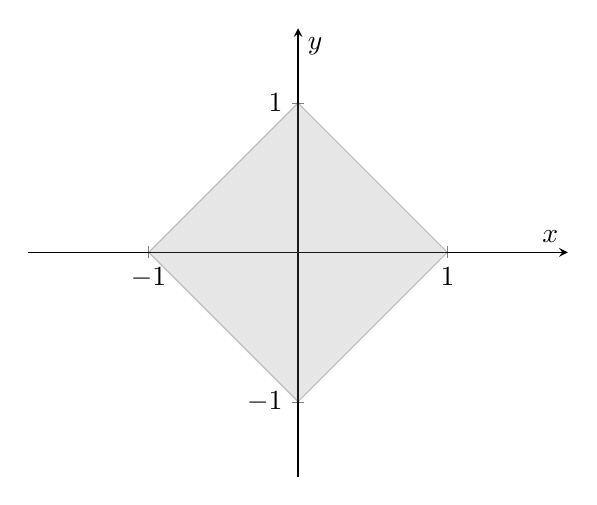
\begin{tikzpicture}
\begin{axis}[my style, xtick = {-1,1}, ytick = {-1,1},
xmin = -1.5, xmax = 1.5, ymin = -1.5, ymax = 1.5]
\draw[rotate around = {45:(0,0)}, fill = gray, opacity = 0.2] (-{sqrt(2)/2},-{sqrt(2)/2}) rectangle ({sqrt(2)/2},{sqrt(2)/2});
\end{axis}
\end{tikzpicture}
\\~\\
For $\|x\| \le 1$: \\ 
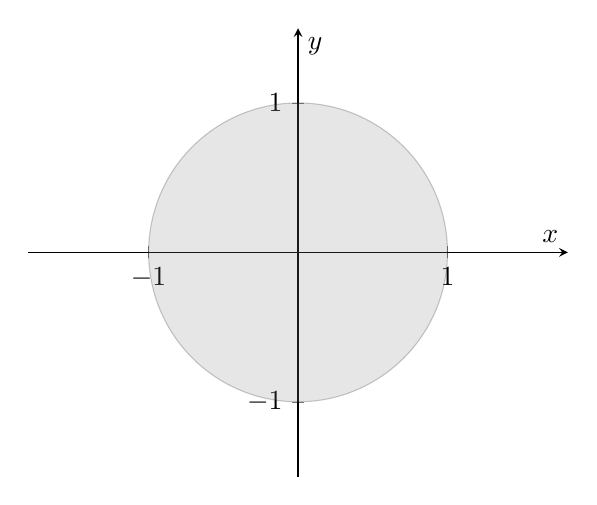
\begin{tikzpicture}
\begin{axis}[my style, xtick = {-1,1}, ytick = {-1,1},
xmin = -1.5, xmax = 1.5, ymin = -1.5, ymax = 1.5]
\draw [fill = gray, opacity = 0.2] (0,0) circle [blue, radius = 1];
\end{axis}
\end{tikzpicture}
\\~\\
For $\|x\|_\infty \le 1$: \\ 
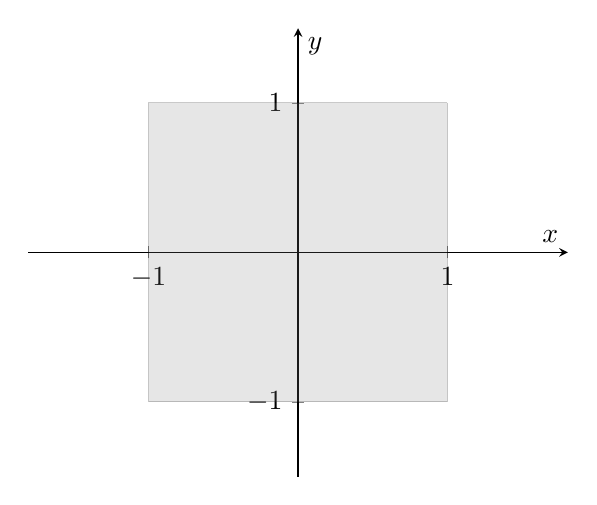
\begin{tikzpicture}
\begin{axis}[my style, xtick = {-1,1}, ytick = {-1,1},
xmin = -1.5, xmax = 1.5, ymin = -1.5, ymax = 1.5]
\draw [fill = gray, opacity = 0.2](1,1) -- (-1,1) -- (-1,-1) -- (1,-1) -- (1,1);
\end{axis}
\end{tikzpicture}
\\
c.
\[
\|x\|_1 = |x_1| + |x_2| + \ldots + |x_N|
\]
\begin{equation*}
\begin{aligned}
\sqrt{N} \cdot \|x\| &= \sqrt{\sum_{i=1}^N 1^2} \cdot \|x\| \\
&= \|(1,1,\ldots, 1) \| \cdot \| x\|\\
&\ge \sum_{i=1}^N |x_i \cdot 1| \\
&= \|x\|_1
\end{aligned}
\end{equation*}
Let $|x_i|$ be the maximum element of $\{|x_1|, |x_2|, \ldots, |x_N| \}$, then
\begin{equation*}
\begin{aligned}
\sqrt{N} \cdot \|x\| &= \sqrt{N} \cdot \sqrt{x_1^2+ x_2^2 + \ldots + x_N^2} \\
&\le \sqrt{N} \cdot \sqrt{x_i^2+ x_i^2 + \ldots + x_i^2} \\
&= \sqrt{N} \cdot \sqrt{N \cdot x_i^2} = N \cdot |x_i| = N \|x\|_\infty
\end{aligned}
\end{equation*}











\end{document}
